\documentclass[pdftex,12pt,xcolor=pdftex,table]{beamer}
%\documentclass[handout,12pt,xcolor=pdftex,table]{beamer}
\synctex=1
\usepackage{comment}
\usepackage{etex}
\usepackage{amsmath}
\usepackage{amsthm}
\usepackage{amsfonts}
\usepackage{amssymb}
\usepackage{latexsym}
\usepackage{mathtools}
\usepackage[english]{babel}
\usepackage[utf8]{inputenc}
\usepackage{tikz}
\usetikzlibrary{calc,matrix,shapes,arrows}
\usepgflibrary{shapes.arrows}
\usepackage[nomessages]{fp}% http://ctan.org/pkg/fp
\newcounter{mycols}
\usepackage{graphicx} % Allows including images
\usepackage{booktabs} % Allows the use of \toprule, \midrule and \bottomrule in tables
\usepackage[sort]{natbib}
\usepackage{bibentry}
\usepackage{layout}
\usepackage[justification=centering,figureposition=bottom]{caption}
\usepackage{longtable}
\usepackage{lscape}
\usepackage{rotating}
\usepackage[figtopcap,center,scriptsize]{subfigure}%[figtopcap]
\usepackage{appendix}
\usepackage{setspace}
\usepackage[multiple,stable]{footmisc}
\captionsetup[longtable]{width=.75\textwidth}

\mode<presentation> {

\usetheme{CambridgeUS}
}

\title{The Right Amount of Trust}
\author{Jeffrey V. Butler, Paola Giuliano \& Luigi Guiso}
\institute{Economic Growth and Comparative Development\\ \textbf{Presented by:} Marcela de Castro \& Juan Camilo Santaella}
\date{\today}

\begin{document}

\begin{frame}
  \titlepage
\end{frame}

\section{Introduction}
\begin{frame}{The Right Amount of Trust}
	\begin{description}
		 \item[\textit{"It can be plausibly argued that much of the economic}]
        \item[\textit{backwardness in the world can be explained by the }] 
		\item[\textit{lack of mutual confidence"}   -Arrow(1972)] 
	\end{description} 
\end{frame}

\begin{frame}{This Paper...}
    \begin{itemize}
    \large 
        \item Does the individual's levels of trust - beliefs held about other's trustworthiness- has any relationship about the economic outcomes?
   \normalsize
	     \item The relationship between \textit{individual} trust and \textit{individual} economic performance is hump-shaped \pause
	            \begin{itemize}
	                \item High trusting individuals tend to assume too much social risk and are cheated more often
	                \item individuals with overly pessimistic beliefs avoid being cheated, but give up profitable opportunities
	            \end{itemize}
	\end{itemize}
\end{frame}

\begin{frame}{This Paper...}
It has been shown that trust is correlated with...
    \begin{itemize}
        \item  GDP per capita and GDP growth. (Knack and Keefer 1996; Knak and Zack 2001; Alan and Cahuc 2010)
        \item firms organization across countries (Bloom et al. 2009) and their ability to grow large (La Porta et al. 1997)
        \item Regulation (Aghion et al. 2010), the size of coutry's stock market (Guiso et al.2008) and cross country trade patterns(Guiso et al.2009) \pause
        \item \textbf{No available research on the individual relationship of trust-income} and its presumable hump-shaped relationship
    \end{itemize}
\end{frame}
\begin{frame}{This Paper...}
    \begin{itemize}
        \item Test the relationship between trust and income using data from the European Social Survey (ESS) \\
            $\qquad \to$ Explore this relationship between individual trust and individual economic performance, particularly at the tails of the distribution of trust beliefs 
        \item \textbf{Findings:}
            \begin{itemize}
                \item Income tends to reach a peak at a level of trust around 7. Beyond a trust level of 7, income declines
            \end{itemize}
    \end{itemize}
\end{frame}
\begin{frame}{This Paper}
    \begin{itemize}
        \item This result cannot be explained by standard forms of reverse causality
        \begin{itemize}
            \item If income causes trust to increase, it can explain the rising portion of the relationship but not the decreasing one, or vice versa
        \end{itemize} \pause
        \item Robust findings about the three main issues of the pooled OLS analysis done with the ESS
         \begin{enumerate}
        \item The humpshaped relationship is identified entirely from individuals who respond 10 to the trust question.
        \item Might be different groups (possibly different by country), not necessarily inverted-U-Shaped relationship.
       \item The result may reflect causality running from income to trust.
    \end{enumerate}
    \end{itemize}
\end{frame}
\begin{frame}{This Paper}
         \begin{enumerate}
        \item The humpshaped relationship is identified entirely from individuals who respond 10 to the trust question.
            \begin{itemize}
                \item Findings suggest that this also holds in countries with low average level of trust
            \end{itemize}
        \item Might be different groups (possibly different by country), not necessarily inverted-U-Shaped relationship.
                \begin{itemize}
                    \item Holds even in a sub group -Swedish data
                \end{itemize}
       \item The result may reflect causality running from income to trust.
                \begin{itemize}
                    \item Study the mechanism through which trust beliefs affect economic performance: Exposure to risk of being cheated using IV for ensuring no reverse causality
                \end{itemize}
    \end{enumerate}
\end{frame}

\section{The Model}
\begin{frame}{A simple model}
    \begin{itemize}
        \item Investor with an endowment $E$
            \begin{itemize}
                \item Decides how much of that investment is invested  in a venture managed by a partner
            \end{itemize}        \pause
        \item The amount $S \leq E$ creates a surplus according to the production function $$f(S)>S$$ \pause
        \item Partner agrees to return a fraction $0< \gamma<1$ to the investor
        \begin{itemize}
            \item Partner can be \textit{honest} -returns promised share of surplus- or a \textit{cheater} -absconds the whole surplus-
        \end{itemize}
    \end{itemize}
\end{frame}
\begin{frame}{A simple model}
    \begin{itemize}
        \item Assumption: Each investor is randomly matched with a partner
        \item A fraction $1-\pi$ of partners are cheaters, the rest is honest but \textbf{investors do not know the real fraction of cheaters in the population}
        \item Investors hold heterogeneous trust beliefs $\tau$, distributed on the unit interval $[0,1]$ about the honesty of the partners
    \end{itemize}
\end{frame}

\begin{frame}{A simple model}
    \begin{itemize}
        \item Given the presence of possibly incorrect beliefs, an investor maximizes a perceived utility given by:
    \begin{equation*}
        \max_{S} Y(S)=E-S +\tau \gamma f(S)
    \end{equation*}
    subject to:
    \begin{equation*}
        S \leq E
    \end{equation*}
    \end{itemize}
\end{frame}

\begin{frame}{A simple model}
    \begin{itemize}
        \item Defining $S_\tau^*$ as the optimal amount invested (i.e. evaluated using true trustworthiness $\pi$), then, $Y(S_\tau^*)$ be the true expected income \pause
    \begin{equation*}
        Y(S_\tau^*)=E-S_\tau^* +\pi \gamma f(S_\tau^*) 
    \end{equation*}
    \item Differentiating $Y(S_\tau^*)$ with respect to the level of trust, $\tau$, yields:
    \begin{equation*}
\frac{\partial Y(S_\tau^*)}{\partial \tau} = \left[\frac{\pi}{\tau} -1\right]\frac{\partial S_\tau^*}{\partial \tau}
\end{equation*}    
    \end{itemize}
\end{frame}

\begin{frame}{A simple model}
    \begin{center}
        \textbf{Theoretical Income-Trust Relationship}
        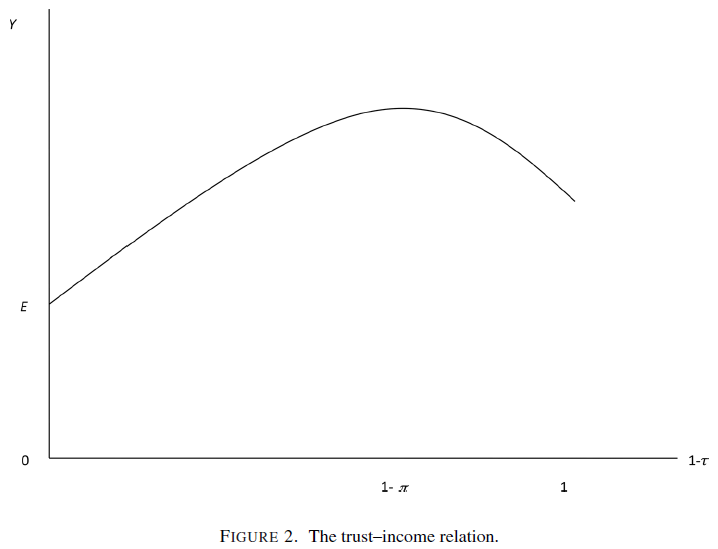
\includegraphics[scale=0.52]{figure_2.PNG}
    \end{center}
\end{frame}

\begin{frame}{A simple model}
\begin{description}
	\large	 \item[Empirical Implications] 
\end{description} 
    \begin{enumerate}
        \item Relationship between individual economic performance and trust beliefs is hump-shaped
        \item The observed Individual's performance $Y(S_\tau^*)$ will, ceteris paribus, peak at a higher level of trust for individuals facing more trustworthy pools of partners
            \begin{itemize}
                \item Since individuals face different pools of partners with different trustworthiness
            \end{itemize} \pause
            %aquí hay que explicar que como los agentes revisan esos errores sobre la confianza en otros y que por eso al tener gente más confiable en general se puede llegar a tener mayor ingreso
     $\quad${\huge \rotatebox{90}{$\dashleftarrow$} } \\ One would expect income to peak at a higher level of $\qquad \qquad \qquad \qquad$ trust in more highly trustworthy counties
    \end{enumerate}
\end{frame}

\section{Data and Empirical Analysis}
\begin{frame}{Data}
    \begin{itemize}
        \item The European Social Survey
        \item Measuring trust:
        \begin{itemize}
            \item “Generally speaking, would you say that most people can be trusted, or that you
can’t be too careful in dealing with people?”
        \end{itemize}
        \item Measuring performance:
        \begin{itemize}
            \item Respondents are asked
to report which income bracket, identified with a letter, best approximates their
household’s total net income.
           \item They identify each bracket with its midpoint.
        \end{itemize}
    \end{itemize}
\end{frame}

\section{Data and Empirical Analysis}
\begin{frame}{Data}
    \begin{itemize}
        \item The SOM Survey
        \item Measuring trust:
        \begin{itemize}
            \item “In your opinion, to what extent can one trust people in general?”
        \end{itemize}
        \item Measuring performance:
        \begin{itemize}
            \item The log of household
income before taxes (defined in brackets).
           \item They identify each bracket with its midpoint.
        \end{itemize}
    \end{itemize}
\end{frame}

\section{Data and Empirical Analysis}
\begin{frame}{Empirical Analysis}
\begin{itemize}
    \item They estimate the following model in the pooled sample of the countries in the ESS:
        \begin{equation*}
        y_{ic} = \sum_j\alpha_jTrust_{jic}+\beta X_{ic} +\delta C+\epsilon_{ic}
        \end{equation*}
    \item $y_{ic}$ is the income in logs of individial i in country c
    \item $X_{ic}$ is a vector of individual controls
    \item $Trust_{jic}$ is a set of ten dummies 
    \item C is a vector of country fixed effects
\end{itemize}
\end{frame}

\section{Data and Empirical Analysis}
\begin{frame}{Empirical Analysis}
    \begin{center}
        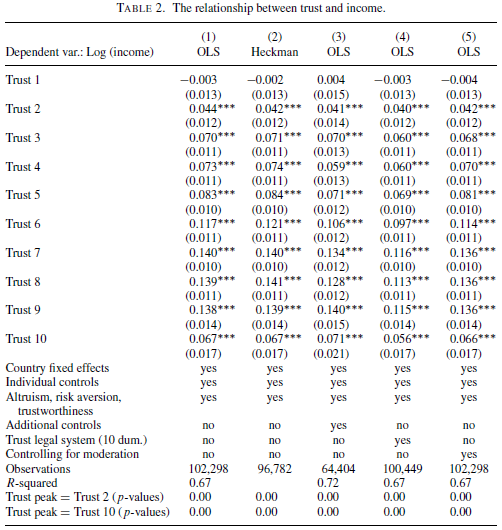
\includegraphics[scale=0.53]{table_2.PNG}
    \end{center}
\end{frame}

\section{Data and Empirical Analysis}
\begin{frame}{Empirical Analysis}
    \begin{center}
            \textbf{The empirical relationship between trust and income.}
        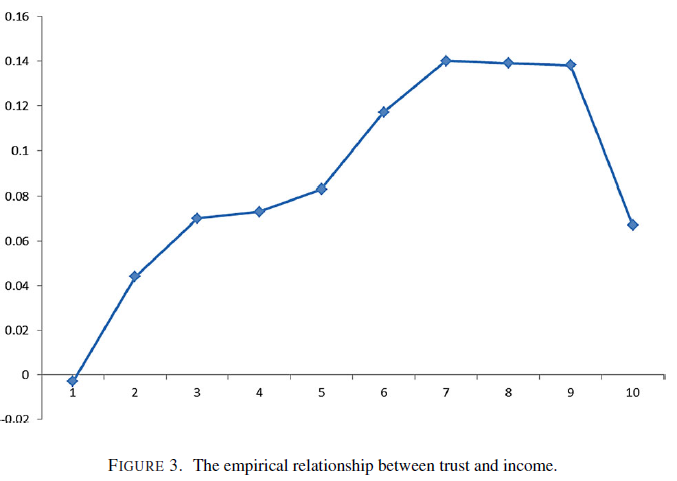
\includegraphics[scale=0.50]{figure_3.PNG}
    \end{center}
\end{frame}

\section{Data and Empirical Analysis}
\begin{frame}{Concerns}
    \begin{enumerate}
        \item The humpshaped
relationship is identified entirely from individuals who respond 10 to the
trust question.
        \item The specification
restricts the trust–income relationship to be the same—and thus generates the same
right level of trust—across individuals.
\item The result may reflect causality running from income to trust.
    \end{enumerate}
\end{frame}

\begin{frame}{Concerns}
\begin{itemize}
    \item Compare observables in the
sample between people reporting a trust level of 10 and people whose level of trust
is equal to the median.
    \item They run separate regressions for low-, average-, and high-trust countries.
    \item They report results using the Swedish data set (A large fraction of people in the upper tail of the trust distribution).
\end{itemize}
\end{frame}

\begin{frame}{Concerns}
    \begin{center}
            \textbf{The empirical relationship between trust and income in low-, average-, and high-trust
countries.}
        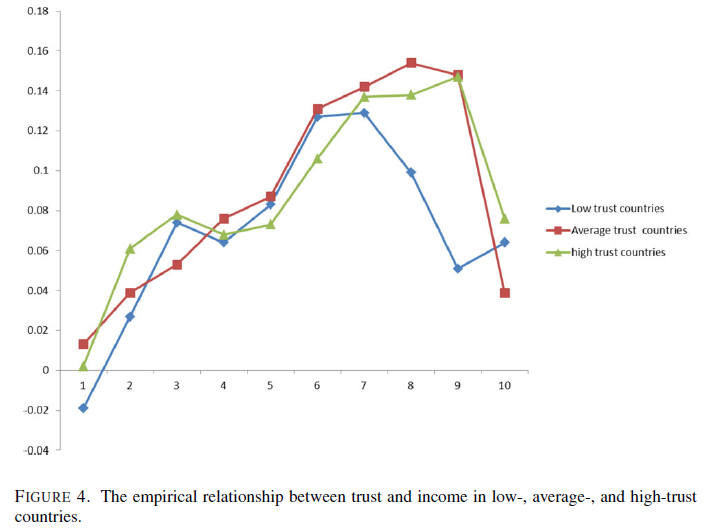
\includegraphics[scale=0.52]{figure_4.PNG}
    \end{center}
\end{frame}

\begin{frame}{Concerns}
    \begin{center}
        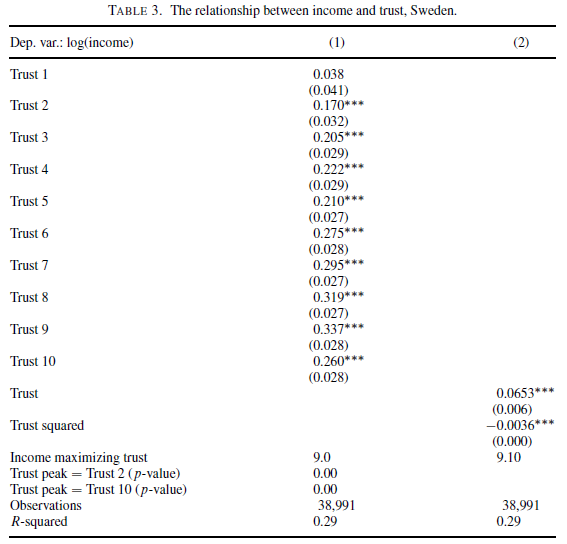
\includegraphics[scale=0.52]{table_3.PNG}
    \end{center}
\end{frame}

\begin{frame}{Concerns}
\begin{itemize}
    \item Reverse causality:
    \begin{itemize}
        \item If reverse causality
argument is true, it cannot explain the declining part of the relationship.
    \end{itemize}
\end{itemize}
\end{frame}

\section{Trust and Cheating}
\begin{frame}{Trust and Cheating}
    \begin{itemize}
        \item Two suboptimal behavior contribute to the hump-shaped income-trust relationship
        \begin{enumerate}
            \item Too much trust undermines performance by increasing the chances of being cheated
            \\ $\dashrightarrow$ The chances of being cheated are increasing in trust \pause
            \item Overly cautions decision making ads to missed profit opportunities
            \\ $\dashrightarrow$ Evidence for this channel is problematic because \underline{missed opportunities are typically unobservable}
        \end{enumerate} \\
    \item Prove the first channel - ESS provide information on how often individuals are being cheated
    \end{itemize}
\end{frame}

\begin{frame}{Measuring Cheating}
    \begin{itemize}
        \item \textbf{Data}
        \begin{itemize}
            \item Second wave of ESS reports information on how often respondents have been cheated by 4 \textbf{domains}: \\
            \textbf{-} Bank/insurance company\\
            \textbf{-} A plumber, builder, car mechanic etc. \\
            \textbf{-} Seller of second-hand goods \\
            \textbf{-} A grocer or food seller\\ \pause
            \item Answers go from never, 1, 2..., 5, 5 or more times
        \end{itemize}
    \end{itemize}
\end{frame}
\begin{frame}{ Number of Times Being Cheated}
    \begin{center}
        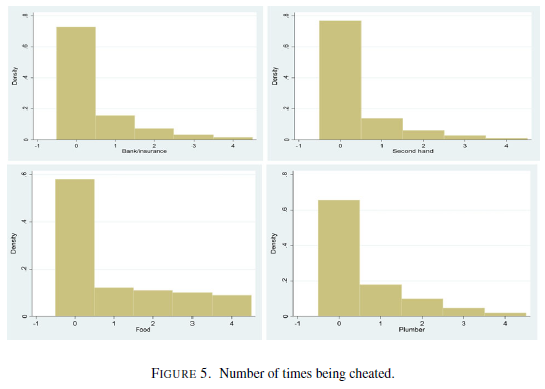
\includegraphics[scale=0.82]{figure_5.PNG}
    \end{center}
\end{frame}

\begin{frame}{Data}
    \begin{itemize}
        \item Construct two summary indicators
        \begin{itemize}
            \item Total number of times being cheated over the four domains
            \item First principal component of the four cheating indicators
        \end{itemize}
    \end{itemize}
\end{frame}
\begin{frame}{Empirical Specification}
    \begin{itemize}
        \item \textbf{Hypothesis:} Chances of being cheated increase with trust
    
    \begin{equation*}
        Z_{ic}^d=\alpha Trust_{ic} + \beta X_{ic} + \gamma C + \epsilon_{ic}
    \end{equation*}
    where $Z_{ic}^d$ is a summary indicator of how often individual $i$ has been cheated in country $C$ in a domain $d$ \pause
    \vspace{0.2cm}
    \item Add a control: risk tolerance
    \end{itemize}
\end{frame}

\begin{frame}{Identification Strategy}
    \begin{center}
        \begin{description}
         \Large \item[Possible Endogeneity]
        \end{description}
    \end{center}
    \begin{itemize}
        \item \textbf{Reverse causality:} Does being cheated affects my trust on others? 
           \begin{itemize}
               \item Yes!! That's their hypothesis - People that is being cheated adjust their trust beliefs
           \end{itemize} \pause
        \item IV approach - Instrument: How much responsibility is delegated to individuals by their supervisors at work
    \end{itemize}
\end{frame}
\begin{frame}{Identification Strategy}
    \begin{center}
        \begin{description}
         \Large \item[Instrument Justification]
        \end{description}
    \end{center}
    \begin{itemize}
        \item Hypothesis: "False consensus" (Ross et al 1977)
            \begin{itemize}
                \item Tendency of individuals to extrapolate the behaviour of others from their own type
            \end{itemize}
        \item If I am trustworthy person, my first guess about other is that they would be trustworthy too. $\to$ my trust on others is based in my own trustworthiness 
    \end{itemize}
\end{frame}
\begin{frame}{Identification Strategy}
    \begin{center}
        \begin{description}
         \Large \item[Instrument Justification]
        \end{description}
    \end{center}
    \begin{itemize}
        \item Hypothesis: "False consensus" (Ross et al. 1977)
            \begin{itemize}
                \item Tendency of individuals to extrapolate the behaviour of others from their own type
            \end{itemize}
        \item If I am a trustworthy person, my first guess about others is that they would be trustworthy too. $\to$ my trust on others is based in my own trustworthiness 
    \end{itemize}
\end{frame}
\begin{frame}{Identification Strategy}
    \begin{center}
        \begin{description}
         \Large \item[Instrument Justification]
        \end{description}
    \end{center}
    \begin{itemize}
        \item \textbf{Relevant:}
           \begin{itemize}
               \item Based on the false consensus hypothesis, it reflects my trust beliefs about others
           \end{itemize} \pause
        \item \textbf{Exogenous:}
           \begin{itemize}
               \item Does not explain why should I change my trust beliefs by my experience of being cheated 
               \item Does not contain individual characteristics that could be associated with the trust beliefs I had before adapting them according to experience
        \end{itemize} \pause
    \end{itemize}
\end{frame}
\begin{frame}{Identification Strategy}
        \begin{center}
        \begin{description}
         \Large \item[Instrument]
        \end{description}
    \end{center}
    \begin{itemize}
        \item How much responsibility is delegated to individuals by their supervisors at work
        \item ESS questions\footnote{Individuals are ask to respond in a scale from zero to ten being ten} about the latitude their manager grants them along:
            \begin{itemize}
                \item Freedom in organizing their daily work
                \item Power to influence policy decisions about the activities of the organization
                \item Freedom to choose or change the pace of their work
            \end{itemize}
    \end{itemize}
\end{frame}
\begin{frame}{}
    \begin{center}
        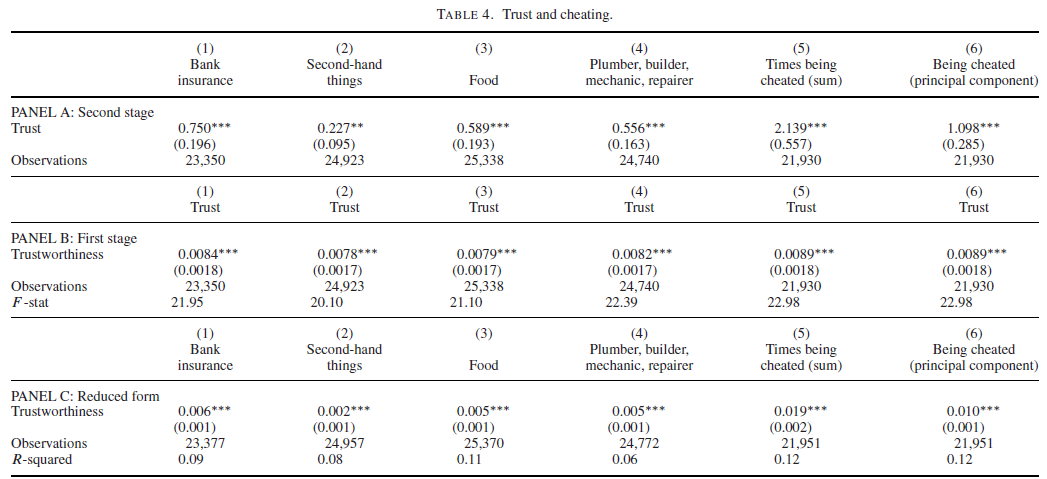
\includegraphics[scale=0.44]{table_4.PNG}
    \end{center}
\end{frame}

\begin{frame}{Trust and Cheating}
    \begin{center}
        \begin{description}
         \Huge \item[Findings]
        \end{description}
    \end{center}
    \begin{itemize}
        \item \textbf{Estimates imply a large effect of trust on exposure to cheating} \pause
        \item Note! \\
        - Results do not show directly that being cheated translates into lost income\\
        - This is suggestive evidence for a potential mechanism driving the trust-income relationship proposed by the authors
    \end{itemize}
\end{frame}
\section{Conclusion}
\begin{frame}{Conclusions}
    \begin{itemize}
        \item Document the existence of a hump-shaped relationship between individual trust and individual income
        \item Excessive trust and excessive mistrust are individually costly
        \begin{itemize}
            \item \textbf{There is a right amount of trust}
        \end{itemize} \pause
        \item The cost of miscalibrated trust beliefs can be substantial $\to$ of the magnitude as returns on education
        \item Mistrust is socially costly as it reduces surplus creation, while excessive trust may create social surplus but may be allocated in a way that harms the overly trusting individuals
    \end{itemize}
\end{frame}
\end{document}

